\chapter{Calorimeter Upgrades
\label{ch:upgrades}}

\section{Phase 1 Simulations}

\subsection{HE Radiation Damage Model}

Radiation damage to the HE plastic scintillator tiles and wavelength-shifting fibers causes a reduction in scintillation light output.
This light loss or darkening is modeled by an exponential degradation function, with specific parameters for each HE tile.
These parameters were derived from 2012 HCAL laser calibration data, which exists for layers 1 and 7.
Figure \ref{fig:laserdatafits} shows exponential fits of relative light yield vs. integrated luminosity in \fbinv from the laser data for selected towers.
The parameter $D$ is a scaling constant for the exponential degradation. A smaller value of $D$ means that the tile darkens more rapidly.
The value of $D$ varies per tile based on the pseudorapidity and layer locations of the tile, which determine the dose received, and also the size of the tile, which determines the mean path length that light must travel to escape the tile.

\begin{figure}[hbtp]
  \begin{center}
    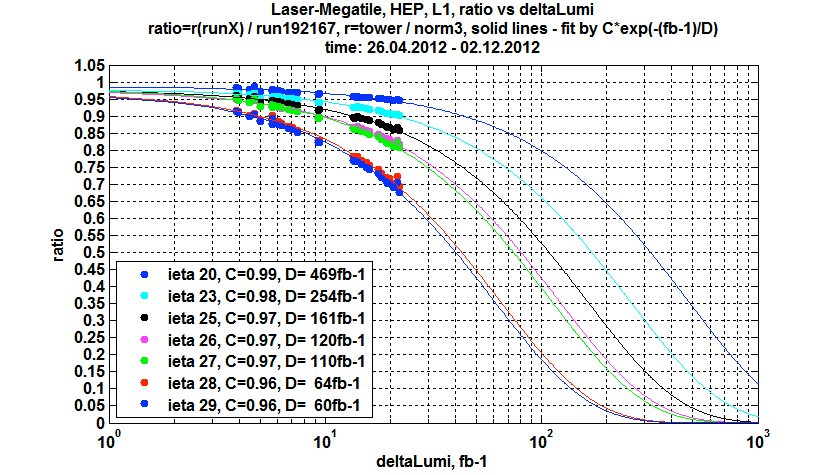
\includegraphics[width=0.49\textwidth]{figures/laserdatafits_HEP_layer1.png}
    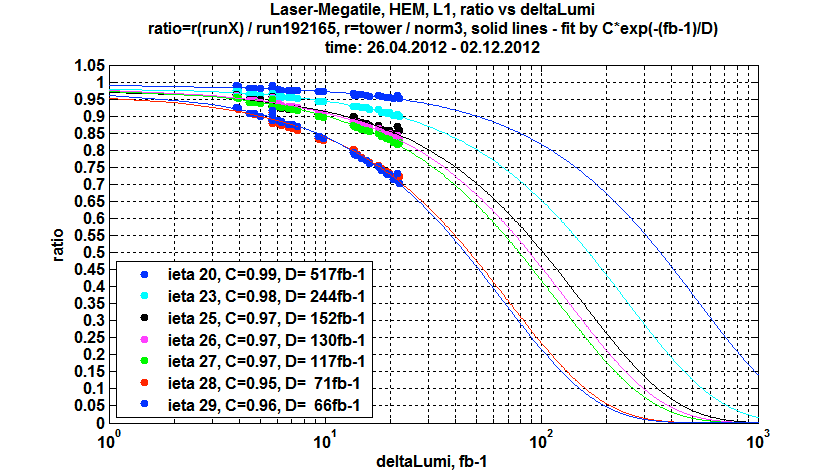
\includegraphics[width=0.49\textwidth]{figures/laserdatafits_HEM_layer1.png}
    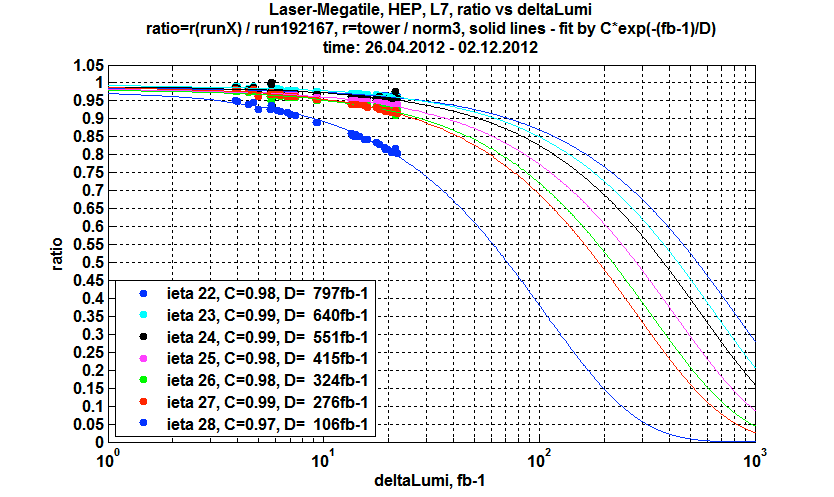
\includegraphics[width=0.49\textwidth]{figures/laserdatafits_HEP_layer7.png}
    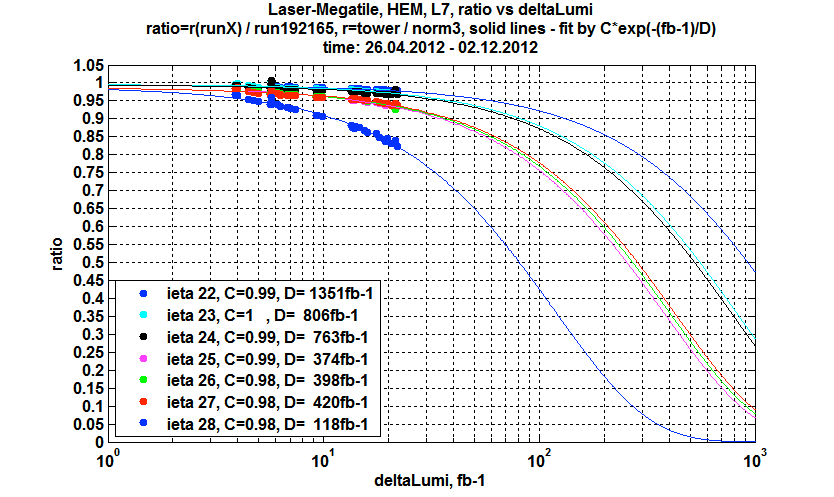
\includegraphics[width=0.49\textwidth]{figures/laserdatafits_HEM_layer7.png}
    \caption{Exponential fits to 2012 HCAL laser calibration data, for layers 1 and 7 in select towers. Data for the positive (HEP) and negative(HEM) sides of the HE are shown separately. The average of the HEP and HEM values for each scaling constant $D$ is used for the radiation damage model.~\cite{epshteyn}}
    \label{fig:laserdatafits}
  \end{center}
\end{figure}

The scaling constants from layers 1 and 7 are interpolated for layers 2-6 and extrapolated for layers 8-17, as shown in Fig. \ref{fig:laserdataconsts}.
The values from layer 1 are used for layers 0 and -1. This specifies a radiation damage model for the entire HE.
Figure \ref{fig:laserdatasignal} shows the relative signal in each layer of each tower of the HE at different integrated luminosity values, based on this radiation damage model. When the LHC center-of-mass energy increases to 14\TeV, a given integrated luminosity value will correspond to a higher amount of dose than it would at 8\TeV when the laser calibration measurements were made. To account for this, the scaling constants are divided by a factor of 1.2, based on FLUKA calculations of the difference in particle flux for 8\TeV and 14\TeV.

\begin{figure}[hbtp]
  \begin{center}
    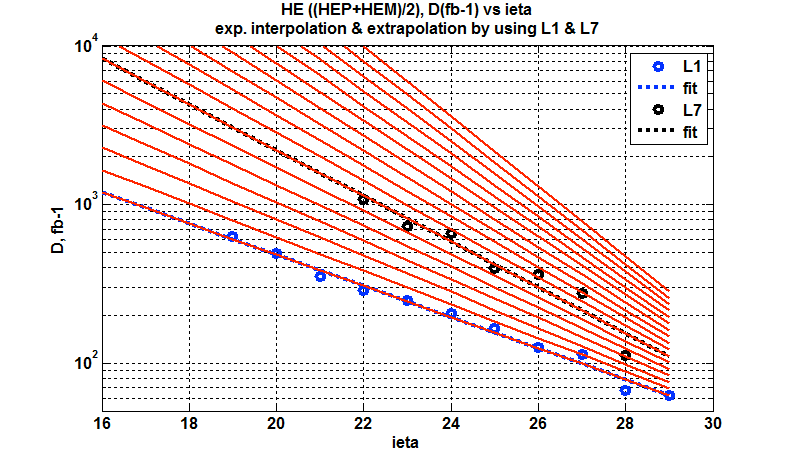
\includegraphics[width=0.98\textwidth]{figures/laserdataconsts.png}
    \caption{Interpolation and extrapolation of the scaling constants $D$ for each layer of each tower in the HE.~\cite{epshteyn}}
    \label{fig:laserdataconsts}
  \end{center}
\end{figure}

\begin{figure}[hbtp]
  \begin{center}
    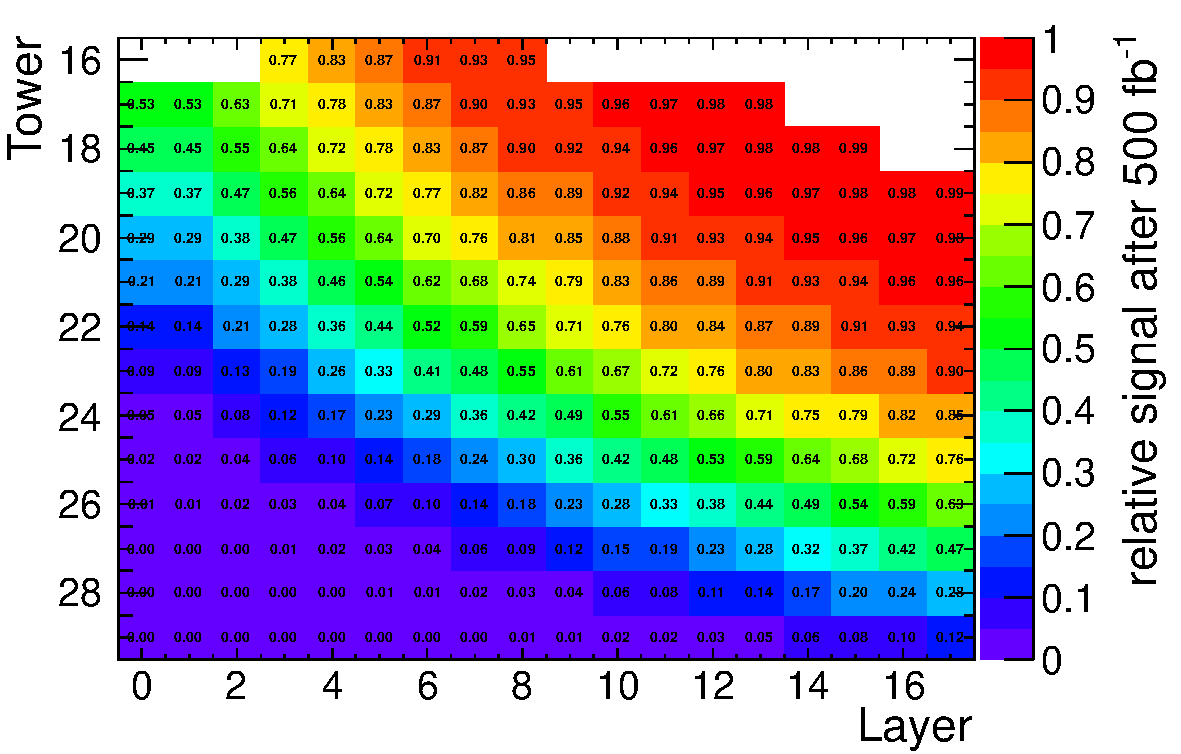
\includegraphics[width=0.98\textwidth]{figures/signal_loss_lumi500.pdf}
    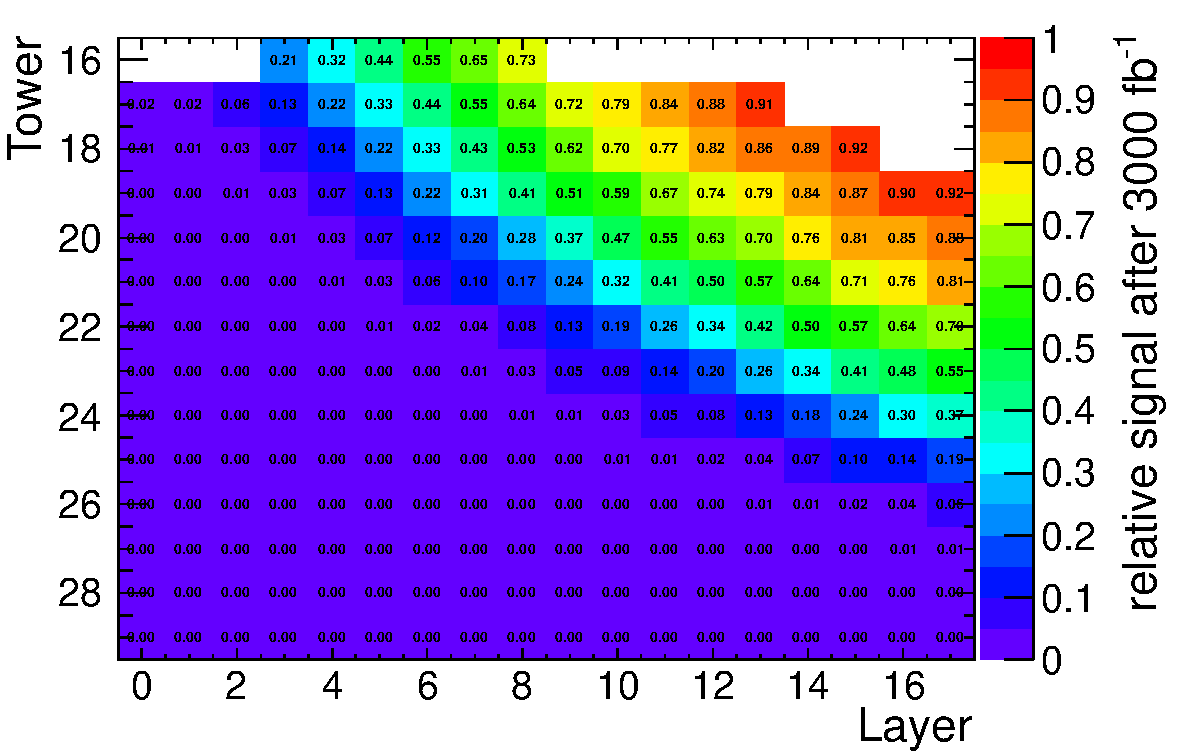
\includegraphics[width=0.98\textwidth]{figures/signal_loss_lumi3000.pdf}
    \caption{Relative signal in each layer of each tower of the HE at (a) 500\fbinv and (b) 3000\fbinv.}
    \label{fig:laserdatasignal}
  \end{center}
\end{figure}

%recalibration factors
The HE photodetectors will be recalibrated to compensate for the darkening of the scintillators and fibers. In a given tower, the light output from several layers is sent to a single photodetector. Each group of layers assigned to a photodetector in this way is called a depth. The specific arrangement of layers into depths, called the depth segmentation scheme, will be changed during the Phase 1 upgrade of the HCAL. Figure \ref{fig:hcaldepths} shows the current depth segmentation scheme and a potential upgrade scheme.

\begin{figure}[hbtp]
  \begin{center}
    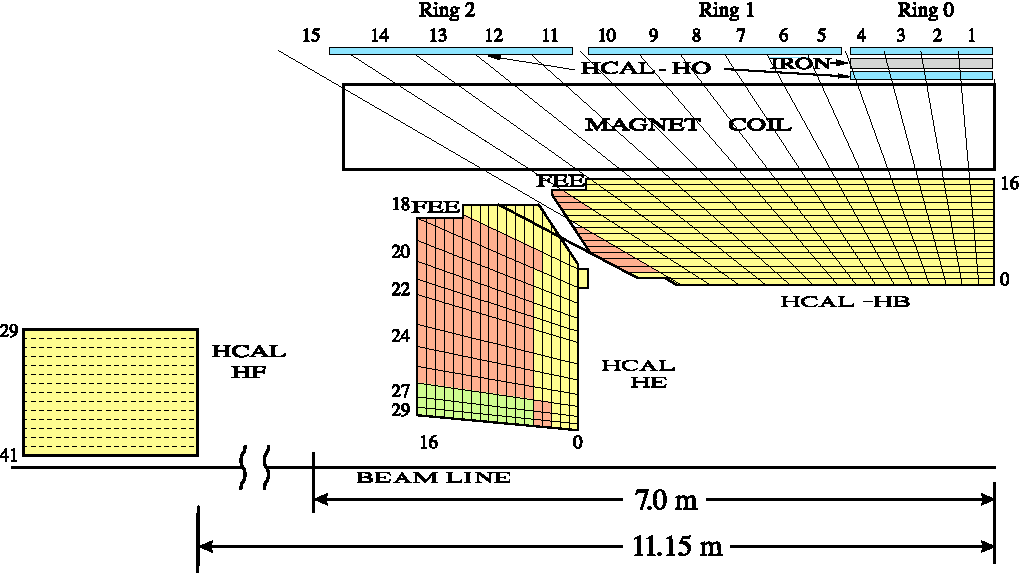
\includegraphics[width=0.49\textwidth]{figures/HCAL-HB-HE-HO-HF.pdf}
    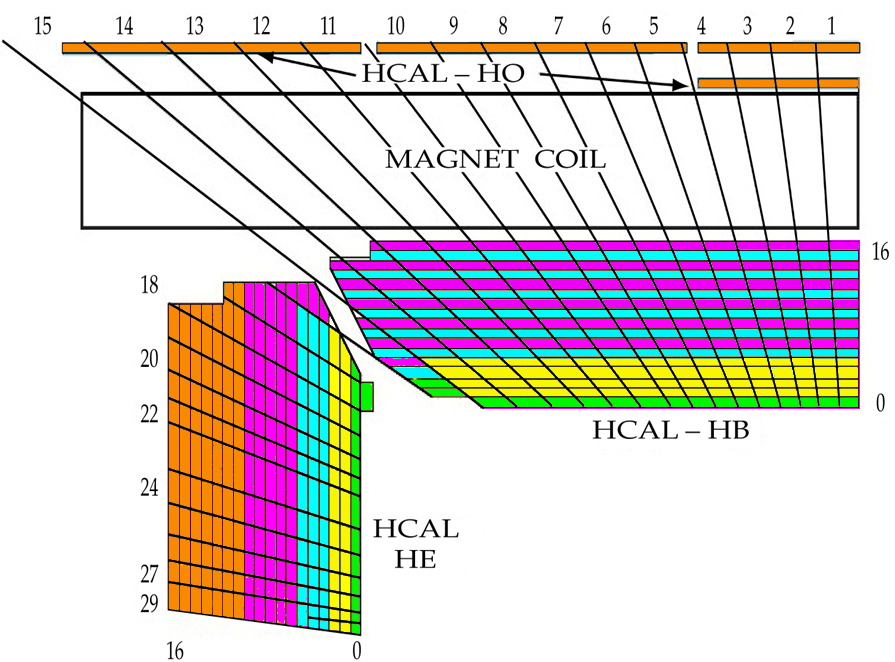
\includegraphics[width=0.49\textwidth]{figures/new_segmentation.png}
    \caption{Depth segmentation schemes in the HCAL for (a) Phase 0 with HPDs as the photodetectors and (b) a proposal for the Phase 1 upgrade with SiPMs as the photodetectors.
			Locations of the front-end electronics (FEE) for the HB and the HE are also shown.~\cite{hcaluptdr}}
    \label{fig:hcaldepths}
  \end{center}
\end{figure}

The HE radiation damage model has a specific degradation curve for each layer of each tower. This means that recalibration factors can be calculated for any depth segmentation scheme, as long as the initial relative weighting of layers within a depth is known. The weighting is determined by tabulating mean energy deposits $\langle E \rangle (\ell,i\eta,0)$ from the full simulation of 100,000 single pion events, where each pion has an energy of 50\GeV and is generated uniformly in $1.6 < \eta < 3.0$ and in $\phi$. The simulation is run at 0\fbinv, so no darkening is simulated. With these mean energy weights, the radiation damage model, and a depth segmentation scheme, recalibration factors can be calculated for any integrated luminosity:
\begin{align}
\langle E \rangle (\ell,i\eta,L) &= e^{-L/D(\ell,i\eta)}\langle E \rangle (\ell,i\eta,0) \label{eq:avgE_layer}\\
\langle E \rangle (d,i\eta,L) &= \sum_{\ell \in d} \langle E \rangle (\ell,i\eta,L) \label{eq:avgE_depth}\\
f(d,i\eta,L) &= \frac{\langle E \rangle (d,i\eta,0)}{\langle E \rangle (d,i\eta,L)} \label{eq:factor_depth}
\end{align}

Equation \eqref{eq:avgE_layer} shows how to use the radiation damage model to find the weights at a given integrated luminosity value, based on the weights at 0\fbinv. Equation \eqref{eq:avgE_depth} is a sum of the weights for the layers in a given depth, determined by the depth segmentation scheme. Equation \eqref{eq:factor_depth} gives the calculation for the recalibration factor at a given depth and integrated luminosity. In these equations, $\langle E \rangle$ is the average energy used as a weight (for layers or for depths), $\ell$ is the layer number, $i\eta$ is the tower number, $L$ is the integrated luminosity in \fbinv, $d$ is the depth number, and $f$ is the recalibration factor.

The recalibration factors for the specified Phase 0 and Phase 1 depth segmentation schemes are shown in Figs. \ref{fig:recalib_phase0} and \ref{fig:recalib_phase1}, respectively. In practice, a maximum recalibration cutoff will be assigned so that photodetector signals and noise are not multiplied by absurdly large values. The default cutoff values are 20 for HPDs and 100 for SiPMs, shown on the figures. %reference the optimization of cutoff values here?

\begin{figure}[hbtp]
  \begin{center}
    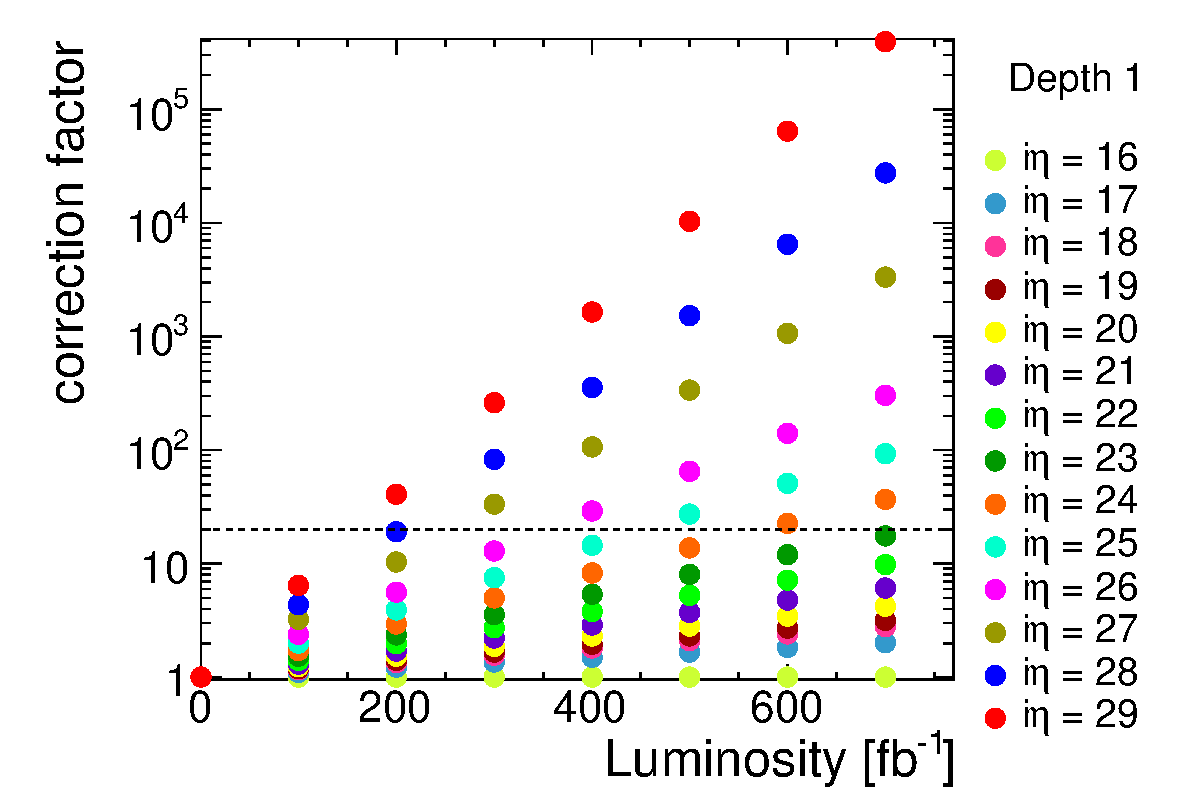
\includegraphics[width=0.49\textwidth]{figures/mean_corr_comp_depth_1_phase0.pdf}
    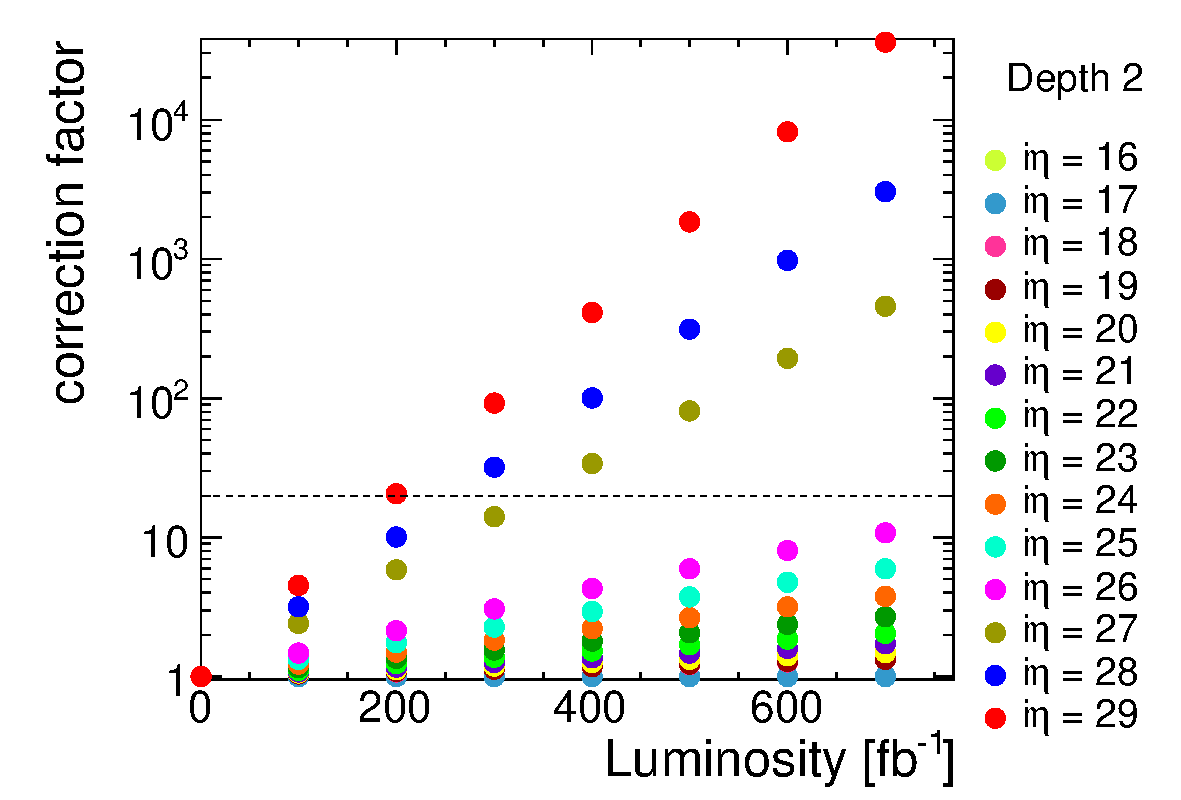
\includegraphics[width=0.49\textwidth]{figures/mean_corr_comp_depth_2_phase0.pdf}
    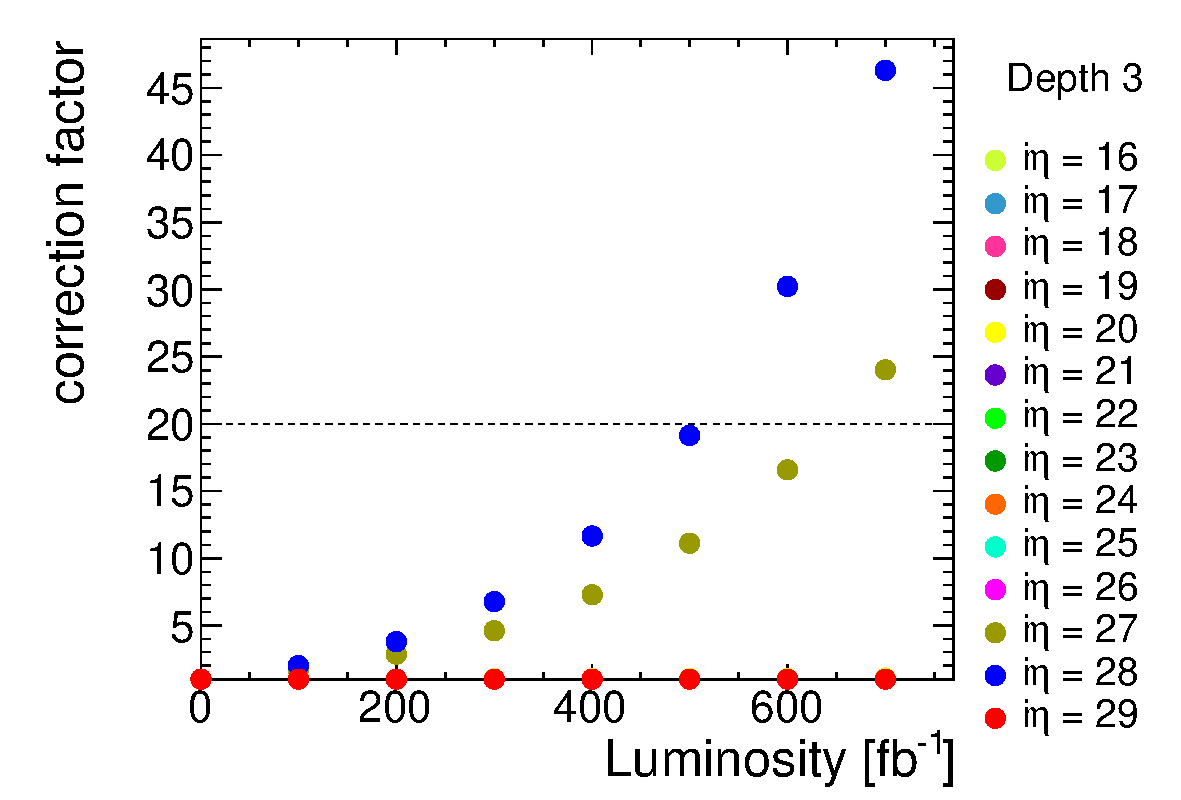
\includegraphics[width=0.49\textwidth]{figures/mean_corr_comp_depth_3_phase0.pdf}
    \caption{Recalibration factors for the Phase 0 depth segmentation scheme. The default recalibration cutoff of 20 is shown as a dotted line on each plot.}
    \label{fig:recalib_phase0}
  \end{center}
\end{figure}

\begin{figure}[hbtp]
  \begin{center}
    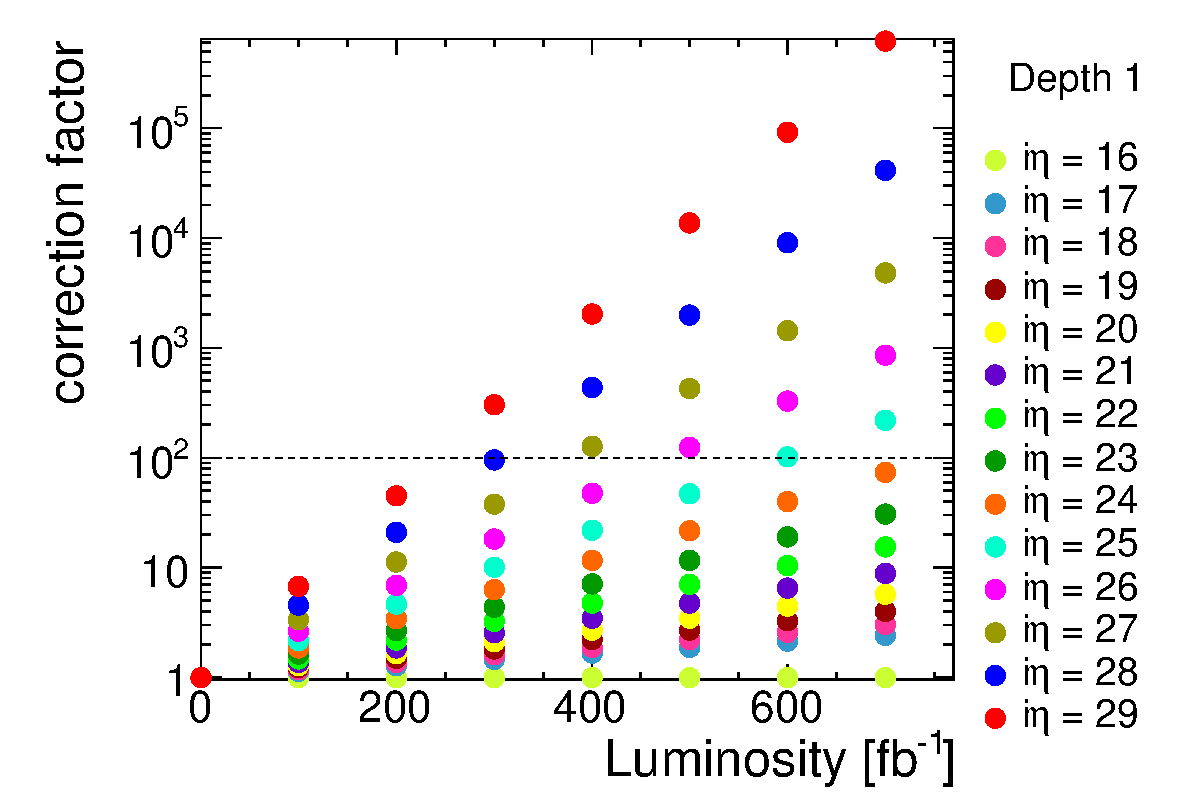
\includegraphics[width=0.49\textwidth]{figures/mean_corr_comp_depth_1_zoom.pdf}
    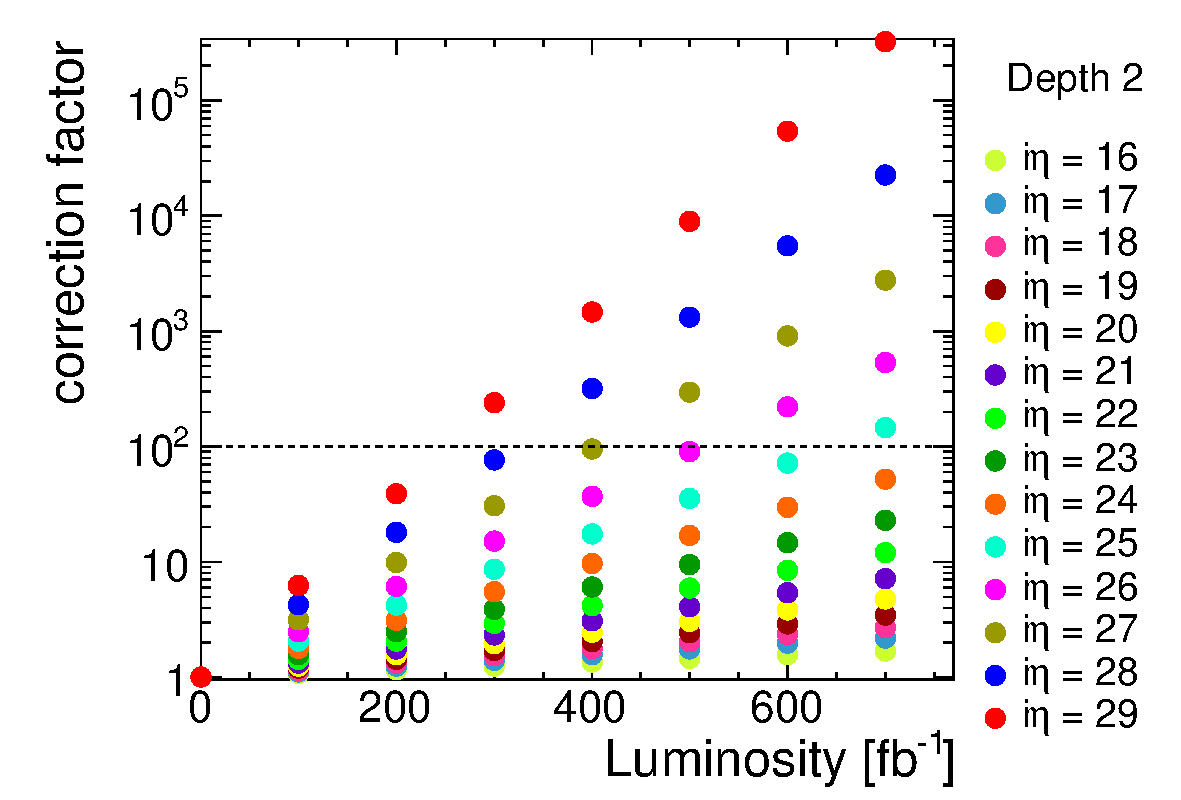
\includegraphics[width=0.49\textwidth]{figures/mean_corr_comp_depth_2_zoom.pdf}
    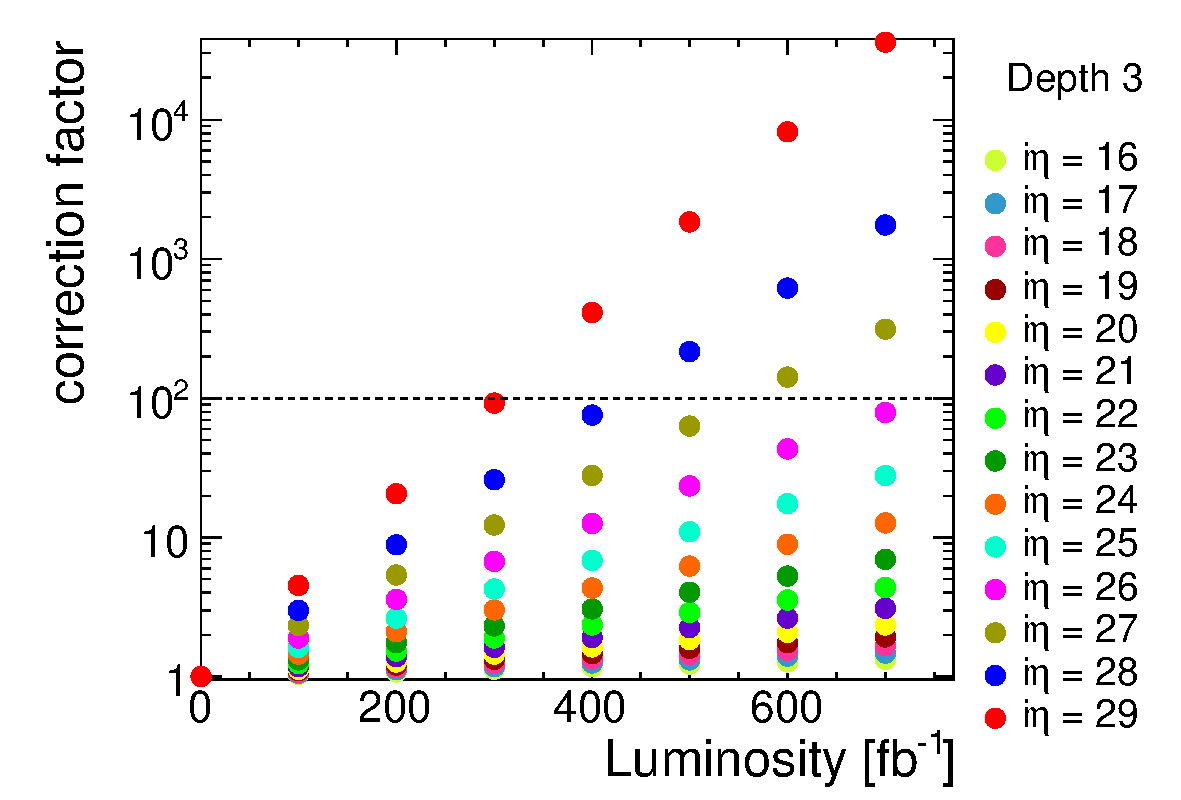
\includegraphics[width=0.49\textwidth]{figures/mean_corr_comp_depth_3_zoom.pdf}
    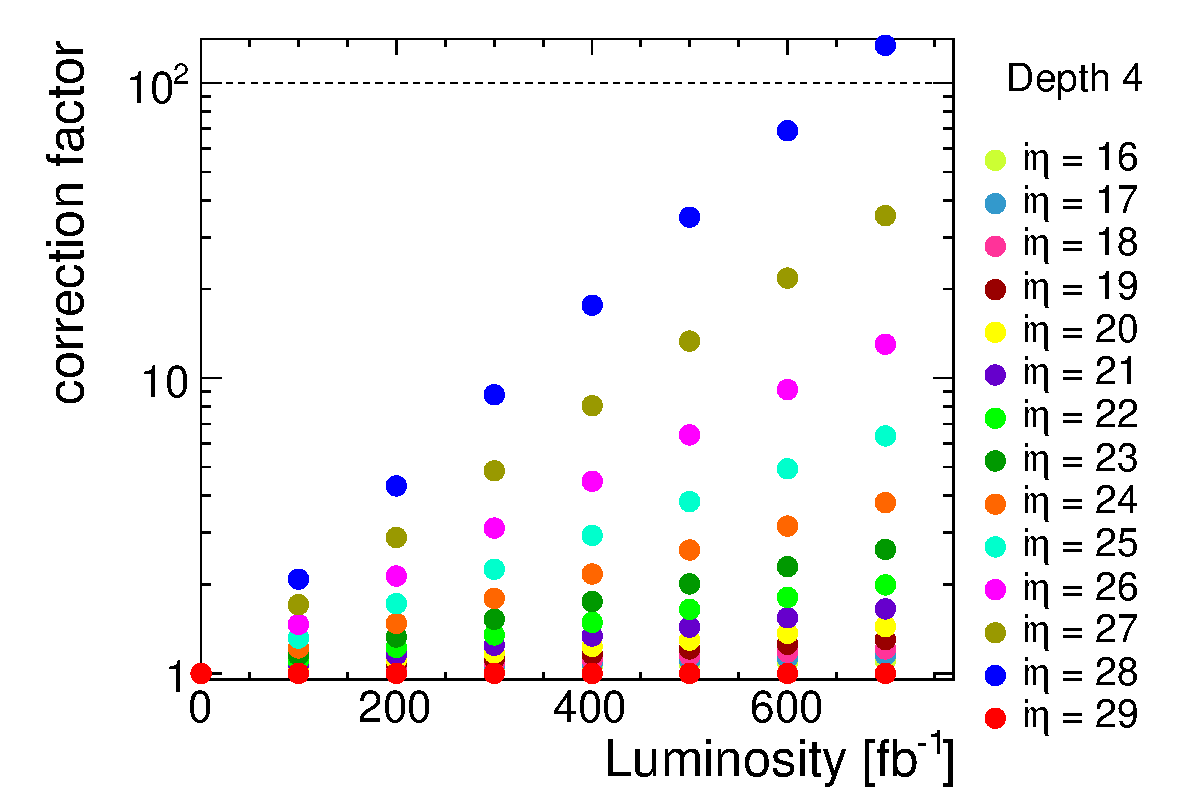
\includegraphics[width=0.49\textwidth]{figures/mean_corr_comp_depth_4_zoom.pdf}
    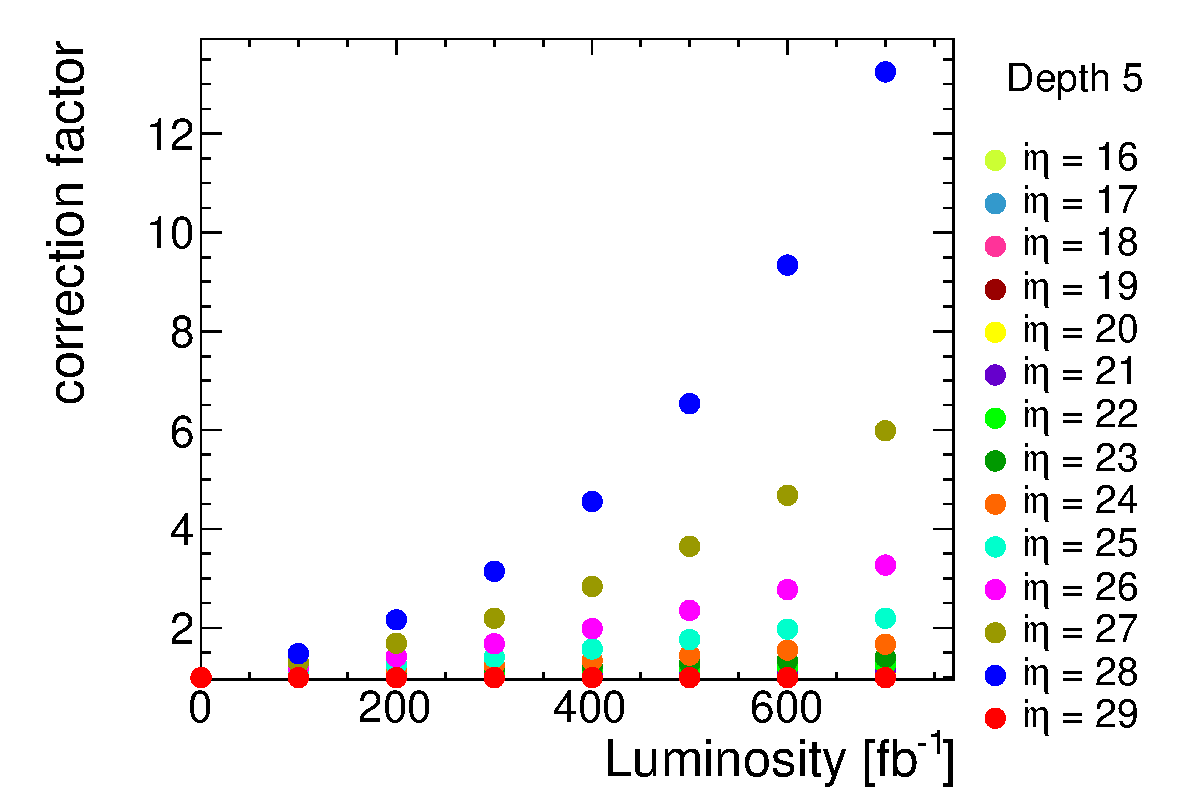
\includegraphics[width=0.49\textwidth]{figures/mean_corr_comp_depth_5_zoom.pdf}
    \caption{Recalibration factors for the proposed Phase 1 depth segmentation scheme. The default recalibration cutoff of 100 is shown as a dotted line on each plot.}
    \label{fig:recalib_phase1}
  \end{center}
\end{figure}

%sipm pedestal widths
Radiation does not have a large effect on the pedestal widths of the HPDs. However, the SIPMs' dark current grows with increasing radiation dose, which leads photodetector noise to increase with integrated luminosity. The simulation of SiPMs accounts for these luminosity-dependent pedestal widths with the following equations, based on measurements shown in Fig. \ref{fig:sipm_darkcurrent}:
\begin{align}
L_{\text{eff}} &= \text{max}(L - 200\fbinv,0) \label{eq:Leff} \\
\sigma_{\text{SiPM}}^{\text{(HB)}} &= 5 + 1.7 \sqrt{L_{\text{eff}}}~\text{[fC]} \label{eq:sipmwidthHB}\\
\sigma_{\text{SiPM}}^{\text{(HE)}} &= 5 + 0.7 \sqrt{L_{\text{eff}}}~\text{[fC]} \label{eq:sipmwidthHE}
\end{align}

Equation \eqref{eq:Leff} accounts for the planned installation of the SiPMs after 200\fbinv have already been collected. Equations \eqref{eq:sipmwidthHB} and \eqref{eq:sipmwidthHE} show the scaling of the pedestal widths with the square root of integrated luminosity. The increase in dark current also changes the pedestal means and zero suppression thresholds, and the simulation accounts for these changes.

\begin{figure}[hbtp]
  \begin{center}
    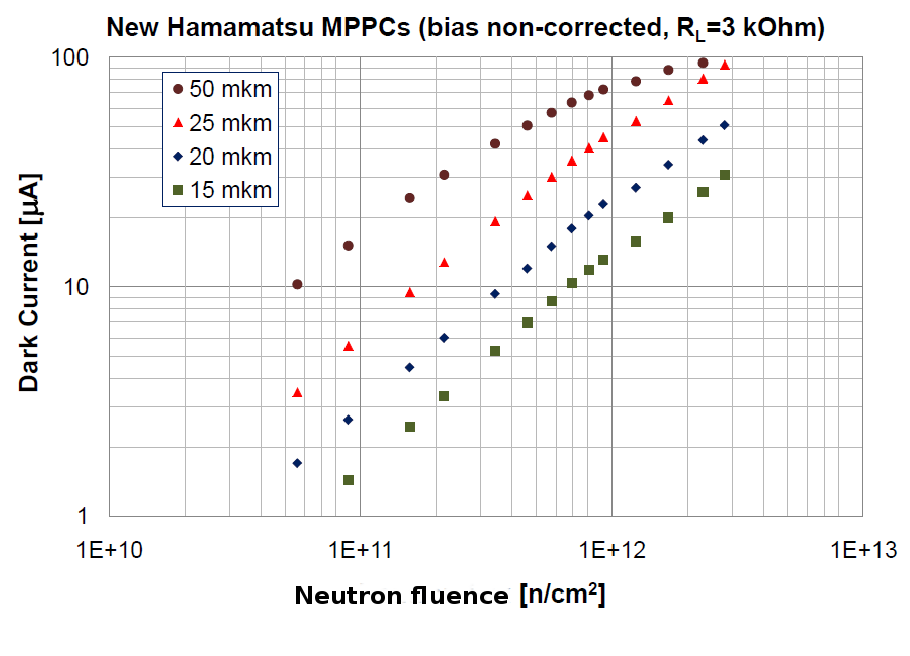
\includegraphics[width=0.98\textwidth]{figures/leakagecurrentneutrons.png}
    \caption{Plot of the SiPM dark current for different radiation doses.~\cite{hcaluptdr}}
    \label{fig:sipm_darkcurrent}
  \end{center}
\end{figure}

\subsection{Jet Studies with Radiation Damage}

\section{Phase 2 Simulations}

\subsection{Validation of Upgrade Standalone Simulation}

\subsection{Tests of Physics Effects on Pion Response and Resolution}

\subsection{HE Rebuild/Extension + Shashlik ECAL Jet Studies}

\section{Hadronic Fast Simulation}

%will be heavily expanded with plots, etc...
\subsection{Retuning of Hadronic Response}

PDF and CDF definitions:
\begin{align}
\int_{-\infty}^{\infty} f(x)dx &= 1 \\
F(x) &= \int_{-\infty}^{x} f(x^{\prime})dx^{\prime} \\
y \equiv F(x) &\rightarrow F^{-1}(y) = x
\end{align}

Parameters:
\begin{align}
\vec{p} &= (\mu,\sigma,a_{L},n_{L},a_{R},n_{R}) \\
d_{L} &= n_{L}/a_{L} \\
d_{R} &= n_{R}/a_{R}
\end{align}

Parameter conditions:
\begin{align}
n_{L}, n_{R} &> 1\\
a_{L}, a_{R} &> 0
\end{align}

Normalization:
\begin{equation}
N = \frac{1}{\sigma\left[\frac{d_{L}}{n_{L}-1} \cdot \text{exp}\left(-\frac{a_{L}^{2}}{2}\right) + \sqrt{\frac{\pi}{2}}\left(\text{erf}\left(\frac{a_{L}}{\sqrt{2}}\right)+\text{erf}\left(\frac{a_{R}}{\sqrt{2}}\right)\right) + \frac{d_{R}}{n_{R}-1} \cdot \text{exp}\left(-\frac{a_{R}^{2}}{2}\right)  \right]}
\end{equation}

Probability density function:
\begin{equation}
f(x;\vec{p}) = N \cdot \begin{cases}
\text{exp}\left(-\frac{a_{L}^{2}}{2}\right) \cdot \left[\frac{1}{d_{L}}\left(d_{L} - a_{L} - \frac{x-\mu}{\sigma}\right)\right]^{-n_{L}} & \text{for $\frac{x-\mu}{\sigma} \leq -a_{L}$} \\
\\
\text{exp}\left(-\frac{1}{2}\left(\frac{x-\mu}{\sigma}\right)^2\right) & \text{for $-a_{L} < \frac{x-\mu}{\sigma} < a_{R}$} \\
\\
\text{exp}\left(-\frac{a_{R}^{2}}{2}\right) \cdot \left[\frac{1}{d_{R}}\left(d_{R} - a_{R} + \frac{x-\mu}{\sigma}\right)\right]^{-n_{R}} & \text{for $\frac{x-\mu}{\sigma} \geq a_{R}$}
\end{cases}
\end{equation}
\newpage

Cumulative distribution function:
\begin{align}
F(x;\vec{p}) &= \sigma N \cdot \begin{cases}
\frac{d_{L}}{n_{L}-1}\text{exp}\left(-\frac{a_{L}^2}{2}\right) \left[\frac{1}{d_{L}}\left(d_{L}-a_{L}-\frac{x-\mu}{\sigma}\right)\right]^{-n_{L}+1} & \text{for $\frac{x-\mu}{\sigma} \leq -a_{L}$} \\
\\
\frac{d_{L}}{n_{L}-1}\text{exp}\left(-\frac{a_{L}^2}{2}\right) + \sqrt{\frac{\pi}{2}}\text{erf}\left(\frac{a_{L}}{\sqrt{2}}\right) + \sqrt{\frac{\pi}{2}}\text{erf}\left(\frac{x-\mu}{\sigma \sqrt{2}}\right) & \text{for $-a_{L} < \frac{x-\mu}{\sigma} < a_{R}$} \\
\\
\frac{d_{L}}{n_{L}-1}\text{exp}\left(-\frac{a_{L}^2}{2}\right) + \sqrt{\frac{\pi}{2}}\text{erf}\left(\frac{a_{L}}{\sqrt{2}}\right)\\
 + \sqrt{\frac{\pi}{2}}\text{erf}\left(\frac{a_{R}}{\sqrt{2}}\right) + \frac{d_{R}}{n_{R}-1}\text{exp}\left(-\frac{a_{R}^2}{2}\right) \\
 + \frac{d_{R}}{1-n_{R}}\text{exp}\left(-\frac{a_{R}^2}{2}\right) \left[\frac{1}{d_{R}}\left(d_{R}-a_{R}+\frac{x-\mu}{\sigma}\right)\right]^{-n_{R}+1} & \text{for $\frac{x-\mu}{\sigma} \geq a_{R}$}
\end{cases}\\
 &= \sigma N \cdot \begin{cases}
B_{L} \left[\frac{1}{d_{L}}\left(d_{L}-a_{L}-\frac{x-\mu}{\sigma}\right)\right]^{-n_{L}+1} & \text{for $\frac{x-\mu}{\sigma} \leq -a_{L}$} \\
\\
A_{L} + C_{L} + \sqrt{\frac{\pi}{2}}\left(1-\text{erfc}\left(\frac{x-\mu}{\sigma \sqrt{2}}\right)\right) & \text{for $-a_{L} < \frac{x-\mu}{\sigma} < a_{R}$} \\
\\
A_{L} + C_{L} + C_{R} + A_{R} \\
 + B_{R} \left[\frac{1}{d_{R}}\left(d_{R}-a_{R}+\frac{x-\mu}{\sigma}\right)\right]^{-n_{R}+1} & \text{for $\frac{x-\mu}{\sigma} \geq a_{R}$} \\
\end{cases}
\end{align}

Inverse cumulative distribution function:
\begin{equation}
x = \begin{cases}
\mu + \sigma \left(-d_{L}\left[\frac{y}{\sigma N}/B_{L}\right]^{\frac{1}{-n_{L}+1}}-a_{L}+d_{L} \right) & \text{for $y < \sigma N A_{L}$} \\
\\
\mu + \sigma \sqrt{2} \text{erfc}^{-1}\left[1-\sqrt{\frac{2}{\pi}}\left(\frac{y}{\sigma N}-A_{L}-C_{L}\right)\right] & \text{for $\sigma N A_{L} \leq y \leq \sigma N (A_{L} + C_{L} + C_{R})$} \\
\\
\mu + \sigma \left(d_{R}\left[\frac{\frac{y}{\sigma N} - A_{L} - C_{L} - C_{R} - A_{R}}{B_{R}}\right]^{\frac{1}{-n_{R}+1}}+a_{R}-d_{R}\right) & \text{for $y > \sigma N (A_{L} + C_{L} + C_{R})$}
\end{cases}
\end{equation}

%Results from Reza should be added here
%Also, remember that there is another section "MIP Energy in Hadronic Fast Simulation"
%but this is only a proposal, not actually implement, so not included here (yet)
\subsection{MIP Fraction in Hadronic Showers}

In the CMS hadronic shower fast simulation, the shower starting depth $s$ is simulated using an exponential distribution. Integrate to find the cumulative distribution for inversion sampling, where $x \in [0,1]$ is a uniformly distributed random number:
\begin{align}
f(s) &= e^{-s}\\
F(s) &= \int_{0}^{s} f(s^{\prime})ds^{\prime} = 1 - e^{-s}\\
x \equiv F(s) &\rightarrow F^{-1}(x) = -\text{ln}(1-x) = \text{ln}\left(\frac{1}{x}\right) = s
\end{align}
In the last step, the fact that $x$ is a uniformly distributed random number in $[0,1]$ is used to take $(1-x) \rightarrow x$.

The condition which decides if the shower will start in ECAL is based on a comparison between the depth of ECAL $d_{\text{ecal}}$ and the starting depth $s$. If the shower does not start in ECAL, the incident hadron is considered to be a MIP (minimum ionizing particle) in ECAL.
\begin{align}
\frac{d_{\text{ecal}}-s}{d_{\text{ecal}}} > 0.1 &\\
\rightarrow 0.9 d_{\text{ecal}} > s &\text{(for pion showers starting in ECAL)} \\
\rightarrow 0.9 d_{\text{ecal}} \leq s &\text{(for pions which are MIPs in ECAL)} \\
\rightarrow d \equiv 0.9 d_{\text{ecal}} &\text{(the minimum starting distance for MIPs)}
\end{align}

Since $f(s)$ is a probability distribution, it has area 1 in $[0,\infty]$. The area for $s = d..\infty$, i.e. when $s \geq d$, should be equal to the probability $p$ that the particle is a MIP. In order to solve this problem, the distribution must be transformed to introduce a free parameter:
\begin{align}
f(s,\lambda) &= \lambda e^{-\lambda s}\\
s &= \frac{1}{\lambda}\text{ln}\left(\frac{1}{x}\right)
\end{align}

Now the integral can be solved to require the correct MIP fraction:
\begin{align}
p = \int_{d}^{\infty} ds \lambda e^{-\lambda s} &= e^{-\lambda d}\\
\rightarrow \lambda &= \frac{1}{d}\text{ln}\left(\frac{1}{p}\right)
\end{align}

Since $d$ is determined by detector geometry, for any $p \in (0,1)$, $\lambda$ can be found to ensure the correct MIP fraction. The final result is just a scaling by $1/\lambda$ of the original equation for randomly generating $s$ from the uniform random number $x$. In practice, $p$ can be determined from full simulation as a function of incident particle energy and $\eta$. The easiest way to do this would be to store values for each $\eta$ and the same energy points that are used in HCALResponse, and then interpolate for intermediate energies. (See Figures \ref{fig:mippct} and \ref{fig:allmippct} for examples.) For energies outside that range, the first or last values should be used rather than extrapolating, since extrapolating could produce $p \leq 0$ or $p \geq 1$, which would create unphysical values of $\lambda$, i.e. $\lambda \not\in (0,\infty)$.

\begin{figure}[hbtp]
\begin{center}
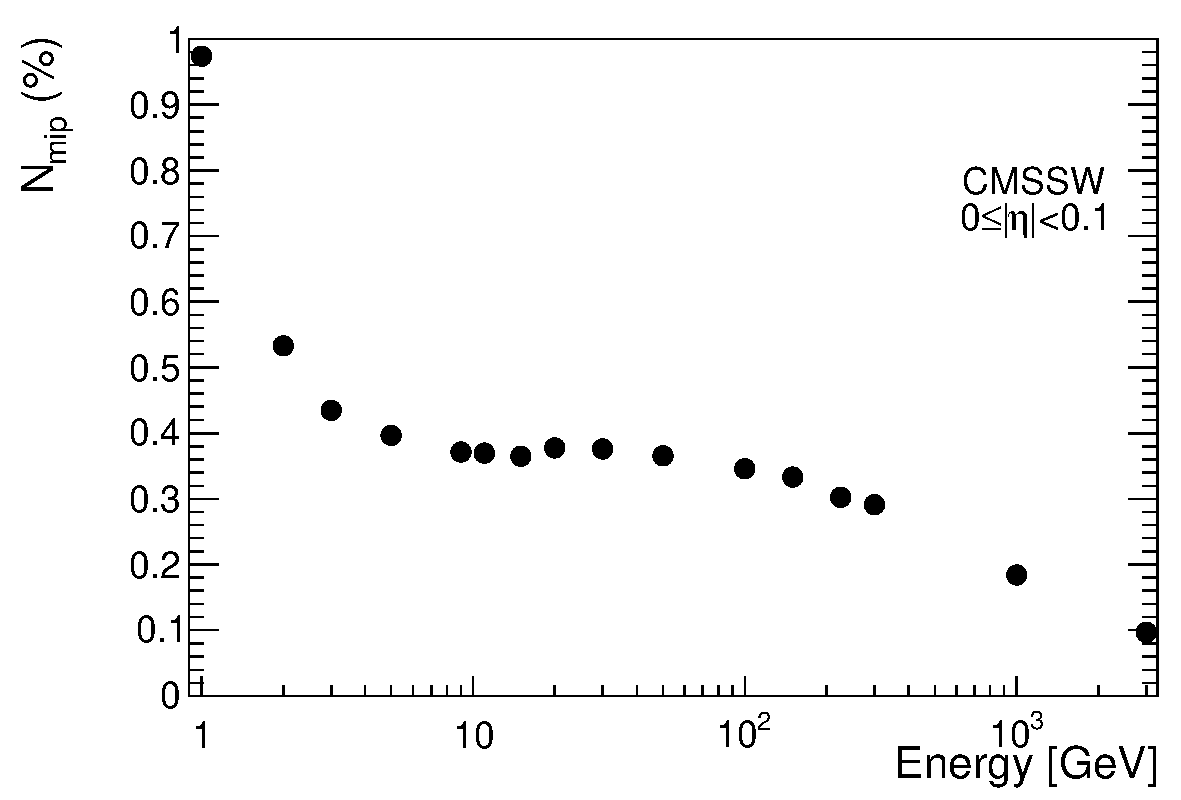
\includegraphics[width=0.49\textwidth]{figures/fs_plot_mip_ieta1.pdf}
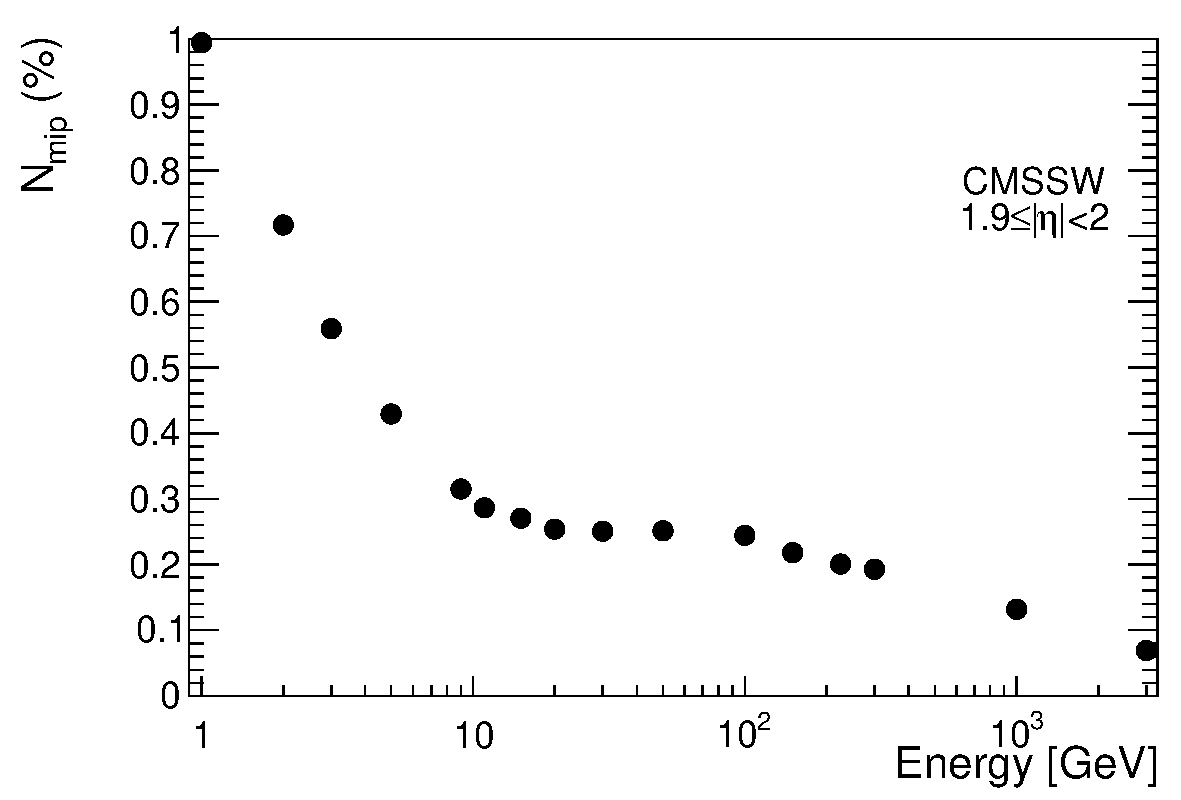
\includegraphics[width=0.49\textwidth]{figures/fs_plot_mip_ieta20.pdf}
\caption{Plots of MIP percentage vs. energy for $i\eta = 1$ (in the barrel) and $i\eta = 20$ (in the endcap).}
\label{fig:mippct}
\end{center}
\end{figure}

\begin{figure}[hbtp]
\begin{center}
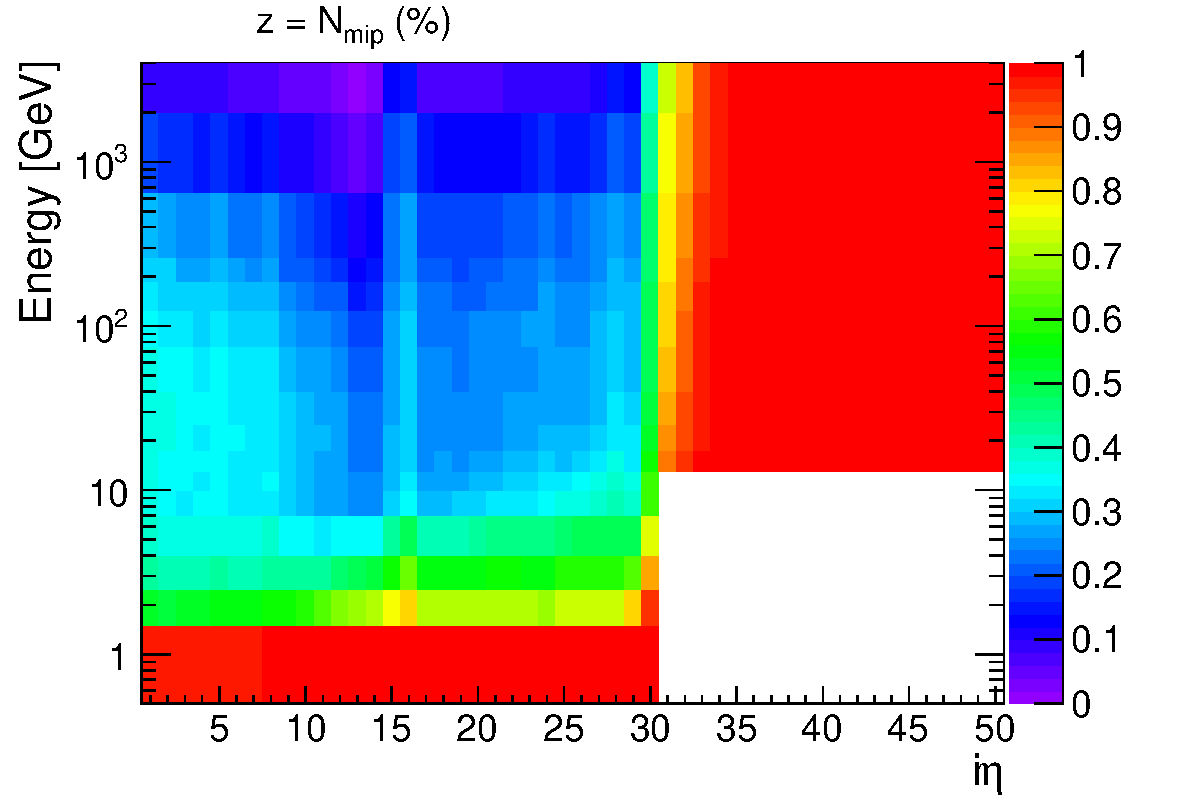
\includegraphics[width=0.95\textwidth]{figures/all_mip.pdf}
\caption{Plots of MIP percentage vs. energy and $\eta$ for the entire calorimeter system.}
\label{fig:allmippct}
\end{center}
\end{figure}

\section{Dose Rate Effects}

\subsection{Dose Rate Effect Models}

\subsection{Scintillator Radiation Damage Studies}